%\documentclass[notes]{beamer}       % print frame + notes
% \documentclass[notes=only]{beamer}   % only notes
\documentclass{beamer}  

\usepackage{wrapfig}
\usepackage{amsmath,amssymb}
%\usepackage[dvipsname]{xcolor}
\usepackage{tikz}
\usepackage{tikz-cd}
\usepackage{graphicx}

\usetikzlibrary{shapes.geometric,shadows,knots}

\tikzset{pics/.cd,
opencube/.style args={#1/#2/#3}{code={
\coordinate (O) at (0,0,0);
\coordinate (A) at (0,#2,0);
\coordinate (B) at (0,#2,#3);
\coordinate (C) at (0,0,#3);
\coordinate (D) at (#1,0,0);
\coordinate (E) at (#1,#2,0);
\coordinate (F) at (#1,#2,#3);
\coordinate (G) at (#1,0,#3);
%% Background
\draw[black,dotted] (O) -- (A);
\draw[black,dotted] (O) -- (C);
\draw[black,dotted] (O) -- (D);
% Forground
\draw[black,dashed] (A) -- (E) -- (F) -- (B) -- cycle;
\draw[black,dashed] (E) -- (D) -- (G) -- (C) -- (B);
\draw[black,dashed] (F) -- (G);

%\draw[black,dashed, blue] (O) -- (A) -- (E) -- (D) -- cycle;
%\draw[black,dashed] (O) -- (A) -- (B) -- (C) -- cycle;
%\draw[black,dashed] (D) -- (E) -- (F) -- (G) -- cycle;
%\draw[black,dashed] (C) -- (B) -- (F) -- (G) -- cycle;
%\draw[black,dashed] (A) -- (B) -- (F) -- (E) -- cycle;

}}}

\tikzset{pics/.cd,
linecube/.style args={#1/#2/#3/#4}{code={
\coordinate (OO) at (0,0,0);
\coordinate (AA) at (0,#2,0);
\coordinate (BB) at (0,#2,#3);
\coordinate (CC) at (0,0,#3);
\coordinate (DD) at (#1,0,0);
\coordinate (EE) at (#1,#2,0);
\coordinate (FF) at (#1,#2,#3);

\coordinate (GG) at (#1,0,#3);
%% Background
\draw[black,dashed] (OO) -- (AA);
\draw[black,dashed] (OO) -- (CC);
\draw[black,dashed] (OO) -- (DD);

\node at (0.5*#1,0.5*#2,0.5*#3) {#4};

% Foreground
\draw[black] (AA) -- (EE) -- (FF) -- (BB) -- cycle;
\draw[black] (EE) -- (DD) -- (GG) -- (CC) -- (BB);
\draw[black] (FF) -- (GG);

%\draw[black,dashed, blue] (O) -- (A) -- (E) -- (D) -- cycle;
%\draw[black,dashed] (O) -- (A) -- (B) -- (C) -- cycle;
%\draw[black,dashed] (D) -- (E) -- (F) -- (G) -- cycle;
%\draw[black,dashed] (C) -- (B) -- (F) -- (G) -- cycle;
%\draw[black,dashed] (A) -- (B) -- (F) -- (E) -- cycle;

}}}


\tikzset{pics/.cd,
shadedcube/.style args={#1/#2/#3/#4/#5}{code={
\coordinate (O) at (0,0,0);
\coordinate (A) at (0,#2,0);
\coordinate (B) at (0,#2,#3);
\coordinate (C) at (0,0,#3);
\coordinate (D) at (#1,0,0);
\coordinate (E) at (#1,#2,0);
\coordinate (F) at (#1,#2,#3);
\coordinate (G) at (#1,0,#3);
\draw[black,fill=#4!80] (O) -- (C) -- (G) -- (D) -- cycle;
\draw[black,fill=#4!30] (O) -- (A) -- (E) -- (D) -- cycle;
\draw[black,fill=#4!10] (O) -- (A) -- (B) -- (C) -- cycle;
\draw[black,fill=#4!20,opacity=0.8] (D) -- (E) -- (F) -- (G) -- cycle;
\draw[black,fill=#4!20,opacity=0.6] (C) -- (B) -- (F) -- (G) -- cycle;
\draw[black,fill=#4!20,opacity=0.8] (A) -- (B) -- (F) -- (E) -- cycle;
\node at (0.5*#1,0.5*#2,0.5*#3) {#5};
}}}
\tikzset{pics/.cd,
gridcube/.style args={#1/#2/#3/#4/#5/#6/#7}{code={
\coordinate (O) at (0,0,0);
\coordinate (A) at (0,#2,0);
\coordinate (B) at (0,#2,#3);
\coordinate (C) at (0,0,#3);
\coordinate (D) at (#1,0,0);
\coordinate (E) at (#1,#2,0);
\coordinate (F) at (#1,#2,#3);
\coordinate (G) at (#1,0,#3);

% Foreground
\draw[fill=#7!20] (A) -- (E) -- (F) -- (B) -- cycle;
\draw[fill=#7!40] (E) -- (F) -- (G) -- (D) -- cycle;
\draw[fill=#7!30] (B) -- (F) -- (G) -- (C) -- cycle;
%\draw[black] (E) -- (D) -- (G) -- (C) -- (B);
%\draw[black] (F) -- (G);

% lines
\foreach \ll in {1,...,#4} {
    \draw[black] (#1/#4*\ll,#2,0) -- (#1/#4*\ll,#2,#3) -- (#1/#4*\ll,0,#3);
}
\foreach \ll in {1,...,#5} {
    \draw[black] (0,#2/#5*\ll,#3) -- (#1, #2/#5*\ll,#3) -- (#1,#2/#5*\ll,0);
}
\foreach \ll in {1,...,#6} {
    \draw[black] (0,#2,#3/#6*\ll) -- (#1,#2,#3/#6*\ll) -- (#1,0,#3/#6*\ll);
}

}}}

%\pgfmathsetmacro{\xx}{0.5}

\mode<presentation>
% \setbeameroption{hide notes}
{
  %\usetheme{Madrid}
  \usetheme{metropolis}
% CSU COLORS
  \definecolor{csugreen}{HTML}{1C674F}
  \definecolor{csugold}{HTML}{B78E00}
    \definecolor{csured}{HTML}{E02F11}

  \definecolor{greenmain}{HTML}{00AF64}
  \definecolor{brick}{rgb}{.85,.1,.2}
  \colorlet{greenstruct}{greenmain!87.5!black}
  \usecolortheme[named=csugreen]{structure}
  % Change this in order to make the presentation look
  % different. Works just like a powerpoint template. 
  % Have your RA mess around until it looks nice.
  \setbeamercovered{dynamic}

  \useinnertheme{rectangles}
  
 %Other colors.

%   \definecolor{bluemain}{HTML}{0B61A4}
%   \definecolor{orangemain}{HTML}{AA6600}
%   \definecolor{redmain}{HTML}{E02F11}
%   \definecolor{redlight}{HTML}{FF9B73}
%   \definecolor{orangelight}{HTML}{FFC373}
%   \definecolor{cmugray}{RGB}{104,104,104}
%   \definecolor{cmulightgray}{RGB}{238,238,238}
%   \setbeamercolor{block body}{bg=cmulightgray}
%   \setbeamercolor{talktitle}{bg=csugreen,fg=white}
%   \setbeamercolor{block title alerted}{bg=csugold}
%   \setbeamercolor{block body alerted}{bg=orangelight}

}
\renewcommand{\footnoterule}{}
\renewcommand{\hat}[1]{\widehat{#1}}
\newcommand{\sourcenum}[3]{$^{\textcolor{bluemain} #1}$\let\thefootnote\relax
  \footnotetext{\begin{flush#2}\textcolor{bluemain}
      {\tiny $^{#1}$ #3}\end{flush#2}}} 
\newcommand{\source}[2]{\let\thefootnote\relax\footnotetext{\begin{flush#1}
      \textcolor{bluemain}{\tiny Source: #2}\end{flush#1}}}  


\DeclareMathOperator{\Span}{Span}
\DeclareMathOperator{\Pres}{Pres}
\DeclareMathOperator{\End}{End}
\newcommand{\bmto}{\rightarrowtail}

\usepackage{wasysym} 
\newcommand{\den}[1]{\Leftcircle\hspace*{-1mm}#1\hspace*{-1mm} \Rightcircle}
\usepackage{listings}

\begin{document}

\title{Group isomorphism is nearly-linear time for most
orders\\ {\small IEEE Foundations On Computer Science FOCS 2021}}
\author{Heiko Dietrich\\ Monash University, Australia\\[10pt] James B. Wilson (presenting)\\ Colorado State University, USA}
\date{February 8, 2022}

\maketitle

%%%%%%%%%%%%%%%%%%%%%%%%%%%%%%%%%%%%%%%%%%%%%%%%%%%%%%%%
\section{Motivation}

\begin{frame}[containsverbatim,fragile]{Outward Facing Motive: honest data types}
Where in this... \\
\begin{center}
\begin{tikzpicture}
\visible<2->{
    \node at (0,0) {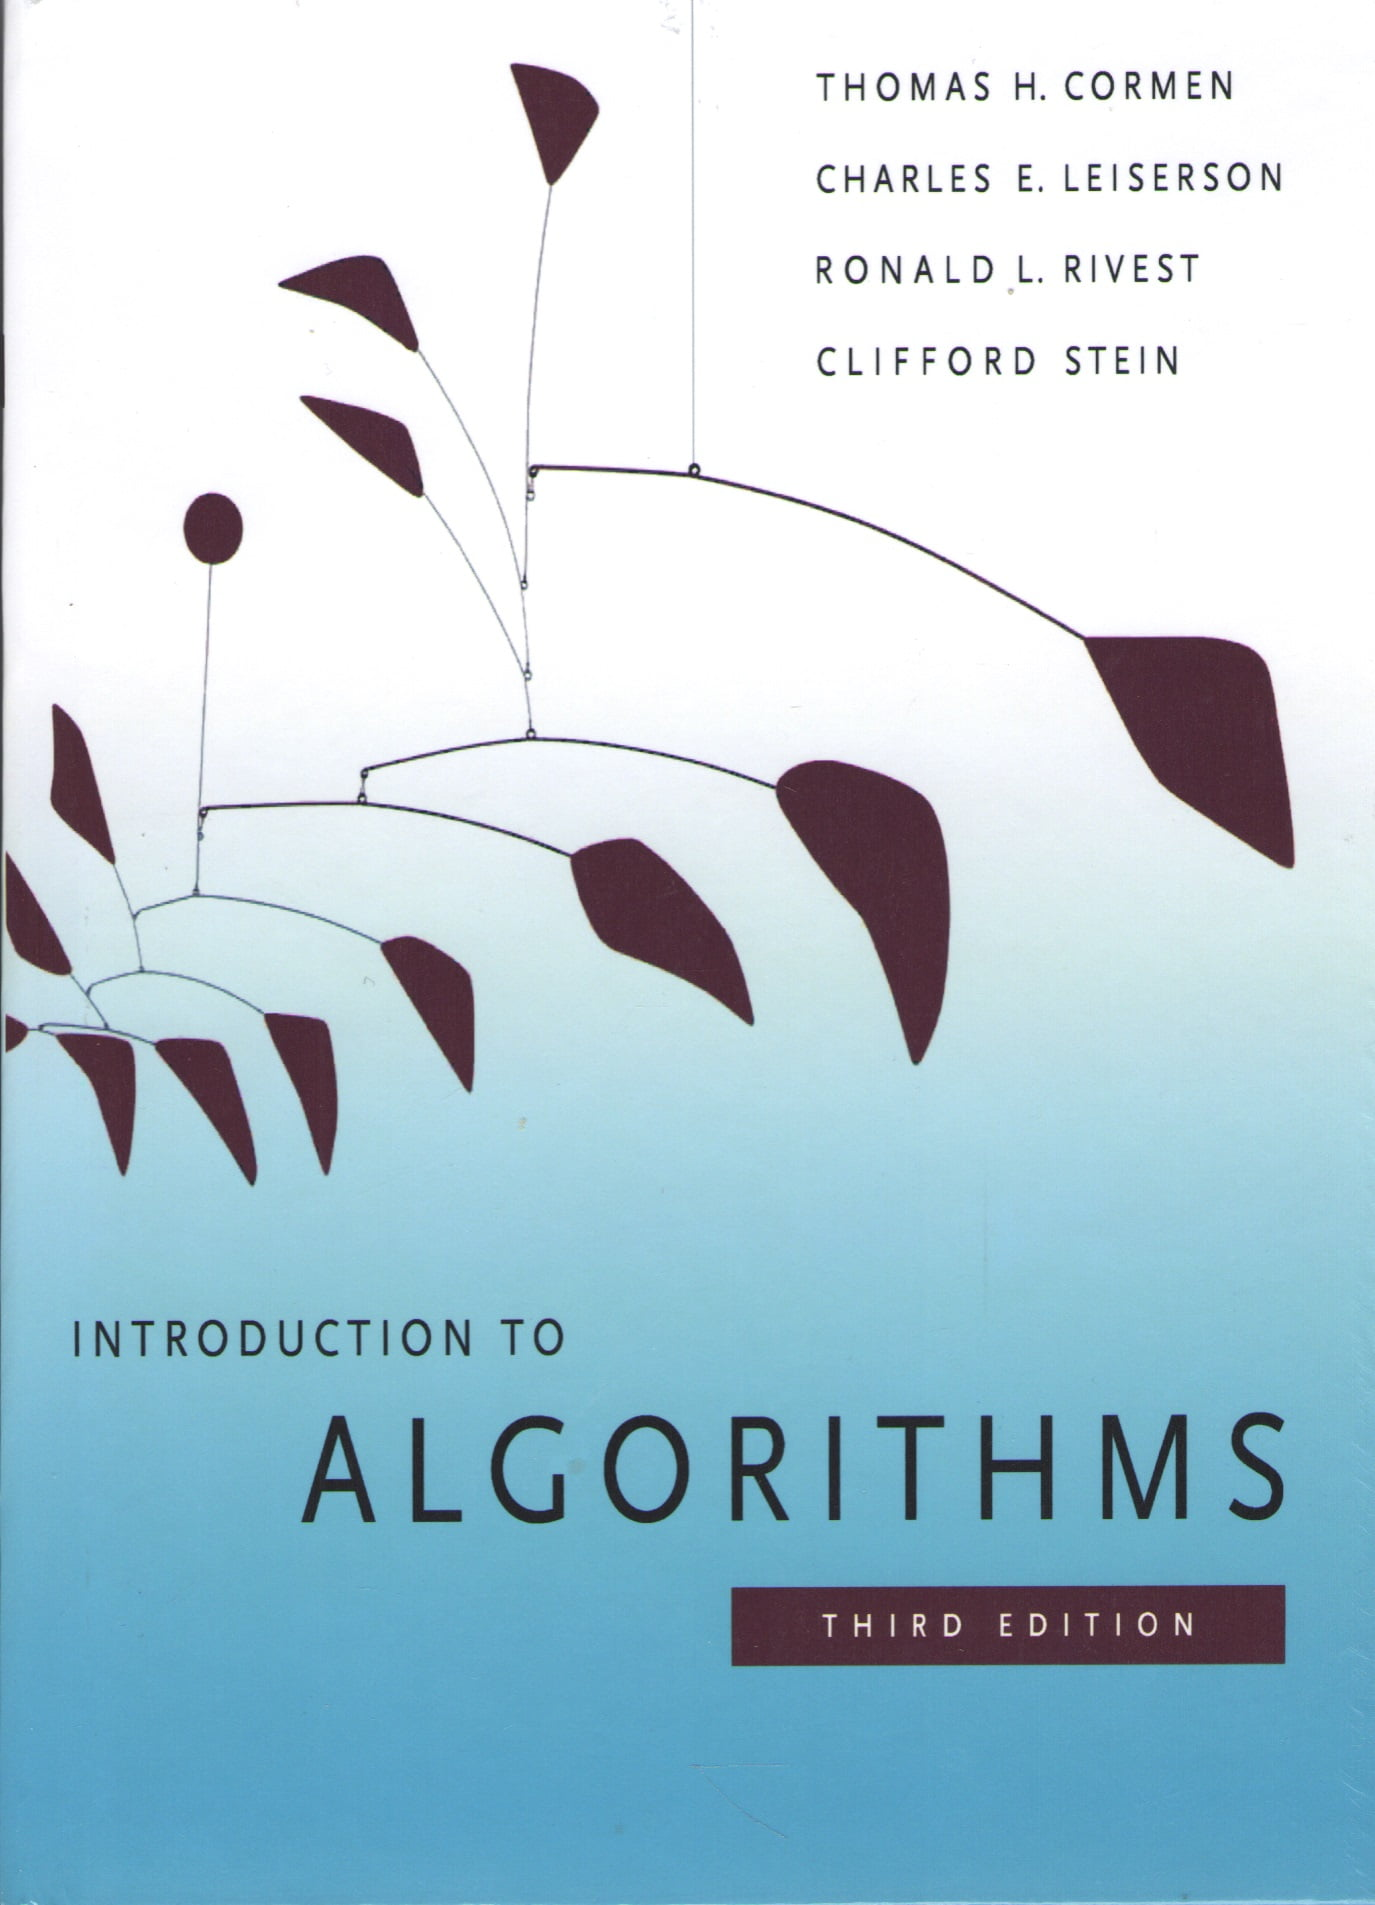
\includegraphics[height=0.25\textheight]{algo.jpg}};
};
\visible<3->{
\node[rotate=30,drop shadow] at (1,1) {
\includegraphics[height=0.25\textheight]{OIP.jpg}};
};
\visible<4->{
\node[rotate=-30,drop shadow] at (3,0.5) {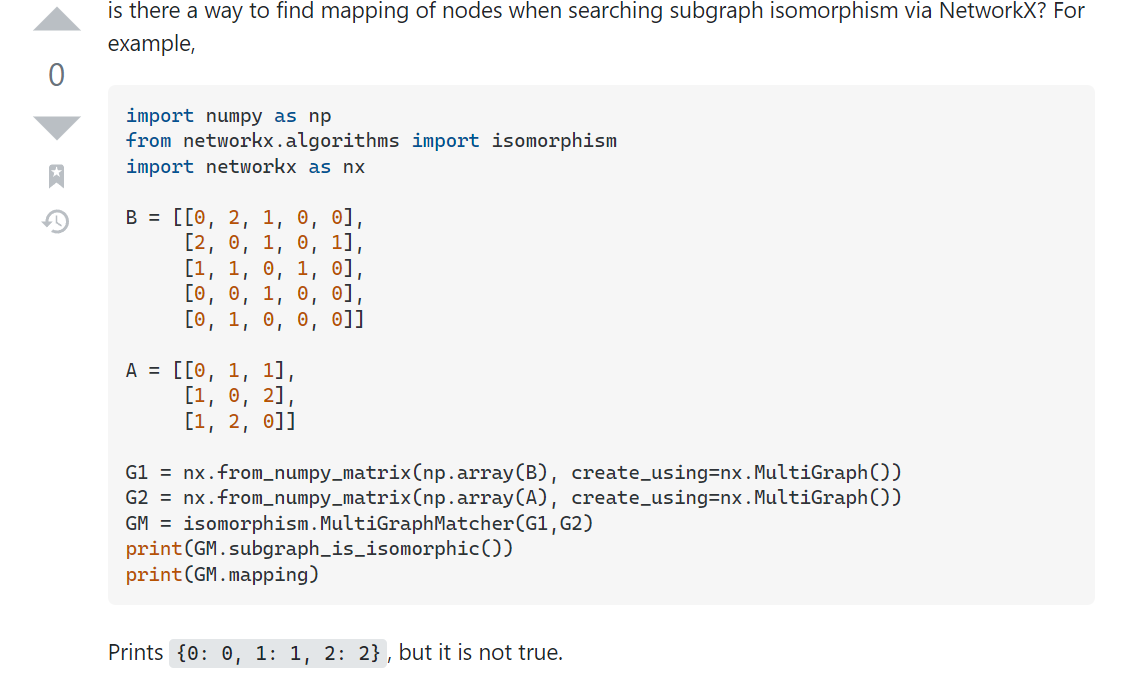
\includegraphics[height=0.25\textheight]{stack.png}};
};
\end{tikzpicture}
\end{center}
\visible<5->{
...do we send people to get help making this... 

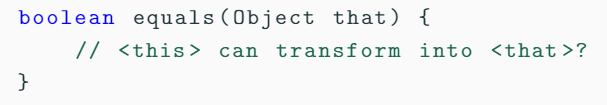
\includegraphics{equals.png}
% \begin{lstlisting}[mathescape=true,language=Java,basicstyle=\ttfamily,commentstyle=\color{csugreen},keywordstyle=\color{blue}]
% boolean equals(Object that) {
%     // <this> can transform into <that>?
% }
% \end{lstlisting}
};
\end{frame}


\begin{frame}{Why groups(oids)?}
\begin{itemize}
    \item \textbf{Transitive}$\to$ \textbf{Partial Multiplication}
    \begin{align*}
    trans_{xyz}:& (x\equiv y) \wedge (y\equiv z) \Rightarrow (x\equiv z)\\
    *:& Eq \times Eq \dashrightarrow Eq
    \end{align*}
\pause

\item  \textbf{Reflexive}$\to$ \textbf{Identity}
    \begin{align*}
    refl_x&: x \Rightarrow  (x\equiv x)\\
    trans_{xxy} &:(x\equiv x)\wedge (x\equiv y) \Rightarrow (x\equiv y)\\
    \hline
    Identity &: refl*evidence  = evidence
    \end{align*}

    \pause
    \item  \textbf{Symmetric}$\to$ \textbf{Inverse}
    \begin{align*}
    sym_{xy}&:(x\equiv y)\Rightarrow (y\equiv x)\\
    trans_{xyx} &: (x\equiv y) \wedge (x\equiv y)  \Rightarrow (x\equiv x)\\
    \hline
    Inverses & : evidence * (evidence)^{-1}  = refl
    \end{align*}
\end{itemize}
\end{frame}
    
\begin{frame}{Anatomy of hard equality}
    \centering
\begin{tikzpicture}[yscale=0.85]
\node at (0,0.5) {$L$};
\node (L) at (0,0) {
    \begin{tikzpicture}[scale=0.5]
        \foreach \brk in {0,1,2} {
        \begin{scope}[rotate=\brk * 240]
            \node[knot crossing, transform shape, inner sep=3pt] (k\brk) at (0,-1) {};
        \end{scope}
        }
        \foreach \brk in {0,1,2} {
            \pgfmathparse{int(Mod(\brk - 1,3))}
            \edef\brl{\pgfmathresult}
            \draw[thick,blue] (k\brk) .. controls (k\brk.4 north east) and (k\brl.4 north west) .. (k\brl.center);
            \draw[thick,blue] (k\brk.center) .. controls (k\brk.16 south east) and (k\brl.16 south west) .. (k\brl);
        }
    \end{tikzpicture}
};

\node at (1.5,0.5) {$\overset{?}{\cong}$};
\node at (3,0.5) {$R$};
\node (R) at (3,0) {
    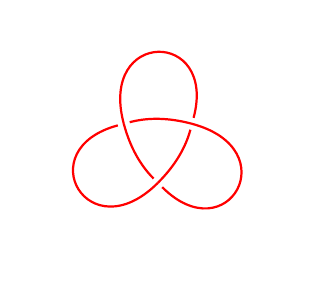
\begin{tikzpicture}[scale=0.5]
        \foreach \brk in {0,1,2} {
        \begin{scope}[rotate=\brk * 120]
            \node[knot crossing, transform shape, inner sep=3pt] (k\brk) at (0,-1) {};
        \end{scope}
        }
        \foreach \brk in {0,1,2} {
            \pgfmathparse{int(Mod(\brk - 1,3))}
            \edef\brl{\pgfmathresult}
            \draw[thick,red] (k\brk) .. controls (k\brk.4 north west) and (k\brl.4 north east) .. (k\brl.center);
            \draw[thick,red] (k\brk.center) .. controls (k\brk.16 south west) and (k\brl.16 south east) .. (k\brl);
        }
    \end{tikzpicture}
};

\visible<2->{
\node (pL) at (-0.5,-3) {$\pi_1(L)=\langle x,y\mid x^2=y^3\rangle$};
\node (pR) at (4.5,-3) {$\pi_1(R)=\langle x,y\mid x^2=y^{-3}\rangle$};
\node[text width=4cm] at (7,-0.5) {Relax category until automorphisms computable.};
\draw[->,thick] (L) to (pL);
\draw[->,thick] (R) to (pR);
};

\visible<3->{
\node (apL) at (0,-5) {$\mathrm{Aut}_{\chi}\pi_1(L)$};
\node (apR) at (3,-5) {$\mathrm{Aut}_{\chi}\pi_1(R)$};
\draw[->,thick] (pL) to[bend right=30] (apL);
\draw[->,thick] (pR) to[bend left=30] (apR);
\node at (2,-3) {$\overset{?}{\cong}$};
\draw[->,thick,dashed] (apL) to[bend right=30] (0.5,-7);
\draw[->,thick,dashed] (apR) to[bend left=30] (2.5,-7);
\node[color=red] at (1.5,-5) {$\not{\cong}_{\chi}$};
\node[text width=4cm] at (7,-5.5) {Recursively refine comparing automorphisms
 with incrementally stricter properties. {\color{red} E.g. respect crossing number $\chi$?}};
};
\end{tikzpicture}

\end{frame}

\begin{frame}{Inward facing Motive: equalivance surveys complexity}
\centering
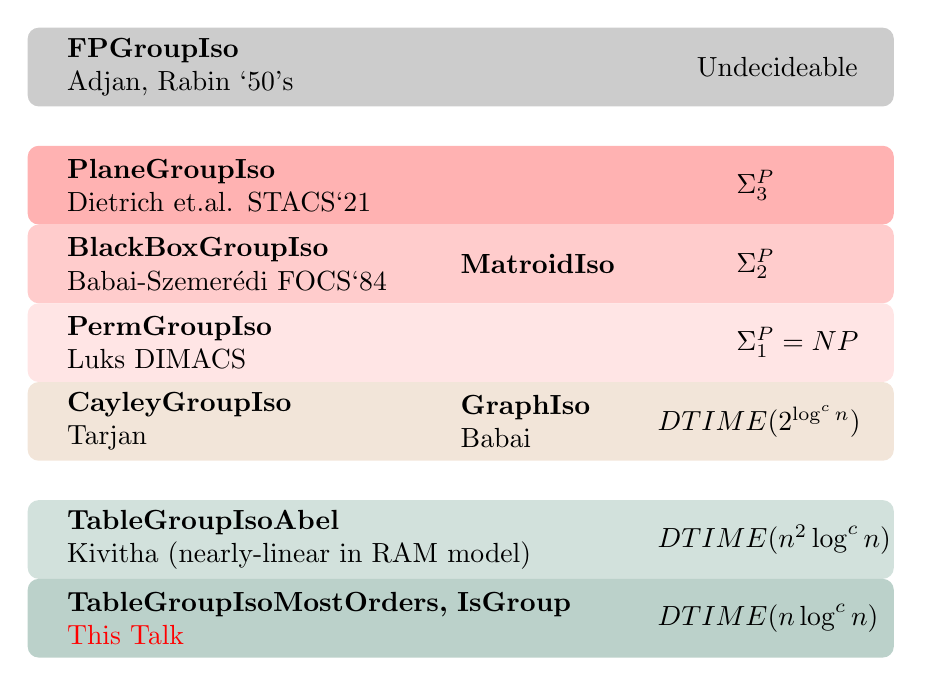
\begin{tikzpicture}

\fill[rounded corners, black!20] (0,5.5) rectangle (11,4.5);
\node[text width=2cm] at (9.5,5) {Undecideable};
\node[text width=3cm] at (2,5) {\textbf{FPGroupIso}\\ Adjan, Rabin `50's};


\fill[rounded corners,red!30] (0,4) rectangle (11,3);
\node[text width=2cm] at (10,3.5) {$\Sigma_3^P$};
\node[text width=5cm] at (3,3.5) {\textbf{PlaneGroupIso}\\ Dietrich et.al. STACS`21};

\fill[rounded corners,red!20] (0,3) rectangle (11,2);
\node[text width=2cm] at (10,2.5) {$\Sigma_2^P$};
\node[text width=5cm] at (3,2.5) {\textbf{BlackBoxGroupIso}\\ Babai-Szemer\'edi FOCS`84};
\node[text width=5cm] at (8,2.5) {\textbf{MatroidIso}};

\fill[rounded corners,red!10] (0,2) rectangle (11,1);
\node[text width=2cm] at (10,1.5) {$\Sigma_1^P=NP$};
\node[text width=5cm] at (3,1.5) {\textbf{PermGroupIso}\\ Luks DIMACS};


\fill[rounded corners,brown!20] (0,1) rectangle (11,0);
\node[text width=2cm] at (9,0.5) {${\tiny DTIME}(2^{\log^c n})$};
\node[text width=5cm] at (3,0.5) {\textbf{CayleyGroupIso}\\ Tarjan};
\node[text width=5cm] at (8,0.5) {\textbf{GraphIso}\\ Babai};

\fill[rounded corners,csugreen!20] (0,-.5) rectangle (11,-1.5);
\node[text width=2cm] at (9,-1) {${\tiny DTIME}(n^2\log^c n)$};
\node[text width=7cm] at (4,-1) {\textbf{TableGroupIsoAbel}\\ Kivitha (nearly-linear in RAM model)};

\fill[rounded corners,csugreen!30] (0,-1.5) rectangle (11,-2.5);
\node[text width=2cm] at (9,-2) {${\tiny DTIME}(n\log^c n)$};
\node[text width=7cm] at (4,-2) {\textbf{TableGroupIsoMostOrders, IsGroup}\\ {\color{red}This Talk}};


\end{tikzpicture}

\end{frame}

\begin{frame}{Schreier-Sims}

    \begin{block}{Problem: Transport}
    \begin{description}
        \item[Given:] A set $\Omega$, allowed permutations $X$, $\omega,\omega'\in\Omega$
        \item[Return:] decide if a string $g$ over $X$ maps $\omega$ to $\omega'$, 
        written $\omega^{g}=\omega'$, and give all such $g$.\footnote{Give words $W$ over $X$
        so that $\omega^h=\omega'$ implies $h=wg$ for a string $w$ over $W$.}
    \end{description}
    \end{block}
\end{frame}



\begin{frame}[fragile]{String Isomorphism}
\begin{center}
    ``Eighth'' == ``HeigHt''
\end{center}
%Cycle right by 1 and replace $h$ with $H$.
\pause
\begin{block}{String Isomorphism}
\noindent
\begin{minipage}{0.6\textwidth}
\noindent
\begin{itemize}
\item {\color{csugreen}\textbf{Given}} strings $s,t:I\to \Sigma$
allowed permutations $G=\langle g_k\rangle\leq \mathrm{Sym}_{I}$, 
$H=\langle h_k\rangle\leq \mathrm{Sym}_{\Sigma}$
\item {\color{csugreen}\textbf{Return}} strings $g=g_{a_1}\cdots g_{a_u}$ 
and $h=h_{b_1}\cdots h_{b_v}$ where $h(s_{i})=t_{g(i)}$; or prove impossible.
\end{itemize}
\end{minipage}
\begin{minipage}{0.3\textwidth}
\begin{tikzcd}
    & I \arrow[d,"g"]\arrow[r, "s"] 
        & \Sigma\arrow[d,"h"] &\\ 
    & I\arrow[r,"t"] & \Sigma & 
\end{tikzcd}
\end{minipage}
\end{block}
\pause

\textbf{Theorem.} (Babai 2016+) If $\Sigma$ fixed, \textsc{StringIso} 
is in Quasipolynomial $n^{O((\log n)^c)}$-time.
\vfill
(\textsc{GraphIso}$\leq_P$ \textsc{StringIso})

\end{frame}

\begin{frame}{Snapshot of solving a hard isomorphism problem}
\centering
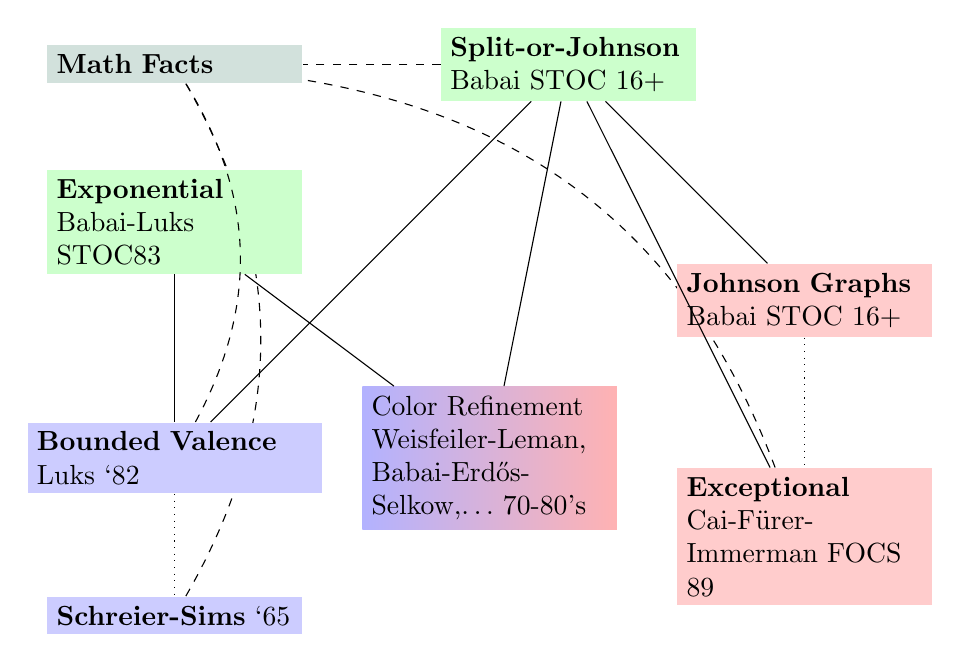
\begin{tikzpicture}
\visible<1->{
\node[fill=csugreen!20,text width=3cm] (math) at (0,5) {\textbf{Math Facts}};
\node[fill=blue!20,text width=3cm] (SS) at (0,-2) {\textbf{Schreier-Sims} `65};
\draw[-,dashed] (SS) to[bend right=30] (math);
};

\visible<2->{
\node[fill=green!20,text width=3cm] (exp) at (0,3) {\textbf{Exponential}\\ Babai-Luks STOC83};
\node[fill=blue!20,text width=3.5cm] (BV) at (0,0) {\textbf{Bounded Valence}\\ Luks `82};
\node[shade, left color=blue!30, right color=red!30,text width=3cm] (color) at (4,0) {Color Refinement\\ Weisfeiler-Leman, Babai-Erd\H{o}s-Selkow,$\ldots$ 70-80's};
\draw[-] (exp) -- (color);
\draw[-] (exp) -- (BV);
\draw[-,dashed] (BV) to[bend right=30] (math);
\draw[-,dotted] (BV) -- (SS);

};

\visible<3->{
\node[fill=red!20,text width=3cm] (CFI) at (8,-1) {\textbf{Exceptional}\\ Cai-F\"urer-Immerman FOCS 89};

\draw[-,dashed] (CFI) to[bend right=30] (math);
};

\visible<4>{
\node[fill=green!20,text width=3cm] (quasi) at (5,5) {\textbf{Split-or-Johnson}\\ Babai STOC 16+};

\node[fill=red!20,text width=3cm] (Johnson) at (8,2) {\textbf{Johnson Graphs}\\ Babai STOC 16+\\};
\draw[-,dotted] (Johnson) -- (CFI);

\draw[-] (quasi) -- (color);
\draw[-] (quasi) -- (BV);
\draw[-] (quasi) -- (Johnson);
\draw[-] (quasi) -- (CFI);
\draw[-,dashed] (quasi) -- (math);
};
\end{tikzpicture}

\end{frame}

%========================================================
\section{Isomorphism of Tables}

\begin{frame}[fragile]{Code Equivalence}

\[\begin{array}{|cc|}
    \hline 
L & i \\ v & e \\
\hline
\end{array}
== 
\begin{array}{|cc|}
    \hline 
E & v \\ i & l \\
\hline
\end{array}\]
\begin{block}{Code Equivalence\footnote{Non-linear twisted, with variable alphabet.}}
\begin{minipage}{0.6\textwidth}
\begin{itemize}
    \item {\color{csugreen}\textbf{Given}} $s,t:I\times J\to \Sigma$, 
    (generators for) permutations 
    $R\leq \mathrm{Sym}_{I}$, 
    $C\leq \mathrm{Sym}_J$, 
    \& $V\leq \mathrm{Sym}_{\Sigma}$ 
    \item {\color{csugreen}\textbf{Return}}  $\sigma\in R$, $\tau\in C$, $\mu\in V$,
    \[\mu(s_{ij}) = t_{\sigma(i)\tau(j)}\] 
\end{itemize}
\end{minipage}
\hfill
\begin{minipage}{0.3\textwidth}
    \begin{tikzcd}
        I \arrow[d,"\sigma"] &[-\dimexpr\pgfmatrixcolumnsep+0.6em\relax]
        \times &[-\dimexpr\pgfmatrixcolumnsep+0.6em\relax] J \arrow[d,"\tau"]
        \arrow[r,"s"] & \Sigma\arrow[d,"\mu"]\\
        I &[-\dimexpr\pgfmatrixcolumnsep+0.6em\relax]
        \times &[-\dimexpr\pgfmatrixcolumnsep+0.6em\relax] J 
        \arrow[r,"t"] & \Sigma
    \end{tikzcd}
\end{minipage}

\end{block}

Babai-Codenotti-Grochow-Qiao $2^{O(n)}$-time bound for constant alphabet $\Sigma$ (SODA `11) \\
Builds on Luks $2^{O(n)}$-hypergraph isomorphism, FOCS `99.

\end{frame}


\begin{frame}[fragile]{Algebra Isomorphism}

\[\begin{array}{|ccccc|}
    \hline 
1 & 2 & 3 & 4 & 5\\
2 & 3 & 4 & 5 & 1\\
3 & 4 & 5 & 1 & 2\\
4 & 5 & 1 & 2 & 3\\
5 & 1 & 2 & 3 & 4\\
\hline
\end{array}
== 
\begin{array}{|ccccc|}
    \hline 
1 & 2 & 3 & 4 & 5\\
2 & 4 & 1 & 5 & 3\\
3 & 1 & 5 & 2 & 4\\
4 & 5 & 2 & 3 & 1\\
5 & 3 & 4 & 1 & 2\\
\hline
\end{array}\]
\begin{block}{Algebra Isomorphism}
\begin{minipage}{0.6\textwidth}
\begin{itemize}
    \item {\color{csugreen}\textbf{Given}} $s,t:I\times I\to I$, 
    (generators for) permutations 
    $G\leq \mathrm{Sym}_I$, 
    \item {\color{csugreen}\textbf{Return}}  $\sigma\in G$,
    \[\sigma(s_{ij}) = t_{\sigma(i)\sigma(j)}\] 
\end{itemize}
\end{minipage}
\hfill
\begin{minipage}{0.3\textwidth}
    \begin{tikzcd}
        I\arrow[d,"\sigma"] &[-\dimexpr\pgfmatrixcolumnsep+0.6em\relax]
        \times &[-\dimexpr\pgfmatrixcolumnsep+0.6em\relax] I \arrow[d,"\sigma"]
        \arrow[r,"s"] & I\arrow[d,"\sigma"]\\
        I &[-\dimexpr\pgfmatrixcolumnsep+0.6em\relax]
        \times &[-\dimexpr\pgfmatrixcolumnsep+0.6em\relax] I
        \arrow[r,"t"] & I
    \end{tikzcd}
\end{minipage}

\end{block}

\end{frame}

\begin{frame}{Group Isomorphism Strategy}

\centering
\begin{tikzpicture}
\visible<1->{
\node[fill=csugreen!20,text width=3cm] (math) at (5,5) {\textbf{Math Facts}};
\node[fill=blue!20,text width=3.5cm] (gt) at (0,-2) {\textbf{Generator Test}\\ Tarjan, Miller STOC78};
\draw[-,dashed] (gt) to[bend right=30] (math);
};

\visible<2->{
\node[fill=csugreen!20,text width=3cm] (data) at (0,5) {\textbf{Data Types}};
\node[fill=blue!20,text width=2cm] (abel) at (0,3) {\textbf{(Nearly) Abelian}\\ Kivitha `07, LeGall};
\node[fill=blue!20,text width=3.5cm] (ss) at (0,0) {\textbf{Semisimplicty}\\ Babai-Codenotti-Qiao ICALP `11};
\node[fill=red!20,text width=3cm] (AT) at (8,2) {\textbf{Adjoint Tensor}\\ Lewis-W. `12};

\draw[-,dashed] (abel) to[bend right=30] (math);
\draw[-,dashed] (ss) to[bend right=30] (math);
\draw[-,dashed] (abel) to[bend right=30] (data);
\draw[-,dashed] (ss) to[bend right=30] (data);
\draw[-,dashed] (color) to[bend right=30] (data);

\draw[-,dashed] (AT) to[bend left=30] (math);

};


\visible<3->{
    \node[fill=red!20,text width=3cm] (TG) at (8,3) {\textbf{Tame Genus}\\ Brooksbank-Maglione-W. `16};    

    \node[shade, left color=blue!30, right color=red!30,text width=3cm] (color) at (4,-2) {\textbf{Tensor Individualization}\\Li-Qiao FOCS17};
    \node[shade, left color=blue!30, right color=red!30,text width=3cm] (cube) at (4,0) {\textbf{Cube free}\\ Dietrich-W. JoA 19};
    
\node[fill=red!20,text width=3cm] (W) at (8,-2) {\textbf{Exceptional}\\ W. ToC 19};
\node[fill=red!20,text width=3cm] (W) at (8,0) {\textbf{Exceptional}\\ Brachter-Schweitzer LICS20};

\draw[-,dashed] (cube) to[bend right=30] (data);
\draw[-,dashed] (W) to[bend left=30] (math);
\draw[-,dashed] (TG) to[bend right=30] (math);
};

\end{tikzpicture}

    
\end{frame}

%==============================================================================
\section{Is it a Group Table?}

\begin{frame}{Promise-to-decision}

A great many computational algebra are analyzed as \textbf{promise problems}
not \textbf{decision problems}.

Identity testing is needed to remove the promise; unsolvable in general (word problem), 
but on tables at least brute-force.
\pause

\begin{block}{Theorem Rajagopalan-Schulman, 2000}
    Given $*:[n]\times [n]\to [n]$, test associativity (and other identities) in
    nearly-linear time $\tilde{O}(n^2)$ in RAM model (constant time ops and
    memory access). Also can test if a group.
\end{block}

\end{frame}

\begin{frame}{RAM-to-TM}

At larger scales Turing Machine (TM) model better match to computations 
that are communication bounded (typical in practice).

RAM -> TM at most a quadratic blow-up.
\begin{block}{Corollary}
Nearly Quadratic-time $\tilde{O}(n^4)$ on multi-tape Turing Machine (TM).
\end{block}

\pause
\begin{block}{Theorem Dietrich-W.}
    Given $*:[n]\times [n]\to [n]$,
    test if a group in time nearly-linear time
    $\tilde{O}(n^2)$ on deterministic multi-tape TM.
    % \footnote{One tape of input length $\ell\in O(n^2)$,
    % and another of length $O(\sqrt{\ell})$.}
\end{block}

\end{frame}

% \begin{frame}{IsGroup Sketch}
% \tikzset{
% mybox/.style={
%     inner sep=0pt,
%     text width=5mm,
%     text height=5mm,
%     align=center,
%     }
% }
% \begin{tikzpicture}
% \node[fill=blue!0, label=center:1,mybox] at  ( 0mm, -0mm) {};
% \node[fill=blue!20,label=center:2,mybox] at  ( 5mm, -0mm) {};
% \node[fill=blue!20,label=center:3,mybox] at  (10mm, -0mm) {};
% \node[fill=blue!30,label=center:4,mybox] at  (15mm, -0mm) {};
% \node[fill=blue!40,label=center:5,mybox] at  (20mm, -0mm) {};
% %
% \node[fill=blue!10,label=center:2,mybox] at  ( 0mm, -5mm) {};
% \node[fill=blue!30,label=center:4,mybox] at  ( 5mm, -5mm) {};
% \node[fill=blue!0, label=center:1,mybox] at  (10mm, -5mm) {};
% \node[fill=blue!40,label=center:5,mybox] at  (15mm, -5mm) {};
% \node[fill=blue!20,label=center:3,mybox] at  (20mm, -5mm) {};
% %
% \node[fill=blue!20,label=center:3,mybox] at  ( 0mm,-10mm) {};
% \node[fill=blue!40,label=center:5,mybox] at  ( 5mm,-10mm) {};
% \node[fill=blue!30,label=center:4,mybox] at  (10mm,-10mm) {};
% \node[fill=blue!10,label=center:2,mybox] at  (15mm,-10mm) {};
% \node[fill=blue!0, label=center:1,mybox] at  (20mm,-10mm) {};
% %
% \node[fill=blue!30,label=center:4,mybox] at  ( 0mm,-15mm) {};
% \node[fill=blue!0, label=center:1,mybox] at  ( 5mm,-15mm) {};
% \node[fill=blue!40,label=center:5,mybox] at  (10mm,-15mm) {};
% \node[fill=blue!20,label=center:3,mybox] at  (15mm,-15mm) {};
% \node[fill=blue!10,label=center:2,mybox] at  (20mm,-15mm) {};
% %
% \node[fill=blue!40,label=center:5,mybox] at  ( 0mm,-20mm) {};
% \node[fill=blue!20,label=center:3,mybox] at  ( 5mm,-20mm) {};
% \node[fill=blue!10,label=center:2,mybox] at  (10mm,-20mm) {};
% \node[fill=blue!0, label=center:1,mybox] at  (15mm,-20mm) {};
% \node[fill=blue!30,label=center:4,mybox] at  (20mm,-20mm) {};
% \end{tikzpicture}

% \end{frame}


\begin{frame}{IsGroup}

\begin{tikzpicture}
    \node at (0,0) {$
        \begin{array}{|c|ccccc|}
        \hline
        \bullet & 1 & 2 & 3 & 4 & 5\\
        \hline
        1 & 1 & 2 & 3 & 4 & 5\\
        2 & 2 & 1 & 4 & 5 & 3\\
        3 & 3 & 5 & 1 & 2 & 4\\
        4 & 4 & 3 & 5 & 1 & 2\\
        5 & 5 & 4 & 2 & 3 & 1\\
        \hline
        \end{array}   
    $};
    \visible<2->{
    \node at (6,0) {$
        \rho(2)  = 
        \begin{array}{|ccccc|}
        \hline
            1 & 2 & 3 & 4 & 5 \\
        \hline 
            2 & 1 & 4 & 5 & 3 \\
        \hline \end{array}    
        =
        (1,2)(3,5,4)
    $};
    };
    \visible<3->{
    \node at (0,-3) {\begin{tikzpicture}
        \node[circle,draw] (1) at (0,0) {1};
        \node[circle,draw] (2) at (2,0) {2};
        \draw[->,thick] (1) to[bend left=30] (2);
        \draw[->,thick] (2) to[bend left=30] (1);
    \end{tikzpicture}};
    \node at (0,-4.5) {$G_{1}=\langle (354)\rangle$};
    };
    \visible<4->{
    \node at (3,-3) {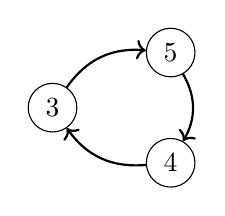
\begin{tikzpicture}
        \node[circle,draw] (3) at (-1,0) {3};
        \node[circle,draw] (4) at (0.5,0.7) {5};
        \node[circle,draw] (5) at (0.5,-0.7) {4};

        \draw[->,thick] (3) to[bend left=30] (4);
        \draw[->,thick] (4) to[bend left=30] (5);
        \draw[->,thick] (5) to[bend left=30] (3);
    \end{tikzpicture}};
    \node at (3,-4.5) {$G_{13}=\{1\}$};
    };
    \visible<5>{
    \node[text width=4cm] at (8,-3) {$|G|=[G:G_1][G_1:G_{13}]$\\ $~=2\cdot 3=6$.\\  Should be 5,\\ not a group.};
    };
\end{tikzpicture}

\end{frame}

    
\begin{frame}{IsGroup}
    \begin{tikzpicture}
        \node at (0,0) {$
        \begin{array}{|c|ccccc|}
        \hline
        * & 1 & 2 & 3 & 4 & 5 \\
        \hline 
        1 & 1 & 2 & 3 & 4 & 5 \\ 
        2 & 2 & 4 & 1 & 5 & 3 \\
        3 & 3 & 5 & 4 & 2 & 1 \\
        4 & 4 & 1 & 5 & 3 & 2 \\
        5 & 5 & 3 & 2 & 1 & 4 \\
        \hline \end{array}    
        $};
        \visible<2->{
        \node at (6,0) {$
            \rho(2)  = 
            \begin{array}{|ccccc|}
            \hline
                1 & 2 & 3 & 4 & 5 \\
            \hline 
                2 & 4 & 1 & 5 & 3 \\
            \hline \end{array}    
            =
            (1,2,4,5,3)
        $};
        };
        \visible<3->{
        \node at (0,-3) {\begin{tikzpicture}
            \node[circle,draw] (1) at (1,0) {1};
            \node[circle,draw] (2) at (0.3,0.8) {2};
            \node[circle,draw] (3) at (-0.6,0.5) {3};
            \node[circle,draw] (4) at (-0.6,-0.5) {4};
            \node[circle,draw] (5) at (0.3,-0.8) {5};

            \draw[->,thick] (1) to[bend right=30] (2);
            \draw[->,thick] (2) to[bend left=30] (4);
            \draw[->,thick] (4) to[bend right=30] (5);
            \draw[->,thick] (5) to[bend right=30] (3);
            \draw[->,thick] (3) to[bend right=30] (1);
        \end{tikzpicture}};
        \node at (0,-4.5) {$|G|=[G:G_{1}|=5$};
        };
        \visible<4>{
        \node[text width=4cm] at (7,-3) {$
        \begin{array}{|c|ccccc|}
        \hline
        * & 1 & 2 & 3 & 4 & 5 \\
        \hline 
        \rho(2)^0 & 1 & 2 & 3 & 4 & 5 \\ 
        \rho(2)^1 & 2 & 4 & 1 & 5 & 3 \\
        \rho(2)^2 & 4 & 5 & 2 & 3 & 1 \\
        \hline \end{array}    
        $\\

        $\rho(2)^2=45231\neq T_4=41532$\\ Not a group.};
        };
    \end{tikzpicture}
\end{frame}

% \begin{frame}{IsGroup}
%     \begin{tikzpicture}
%         \node at (0,0) {$
%         \begin{array}{|c|ccccc|}
%         \hline
%         * & 1 & 2 & 3 & 4 & 5 \\
%         \hline 
%         1 & 1 & 2 & 3 & 4 & 5 \\ 
%         2 & 2 & 4 & 1 & 5 & 3 \\
%         3 & 4 & 5 & 4 & 2 & 1 \\
%         4 & 4 & 1 & 5 & 3 & 2 \\
%         5 & 5 & 3 & 2 & 1 & 4 \\
%         \hline \end{array}    
%         $};
%         \visible<2->{
%         \node at (6,0) {$
%             \rho(2)  = 
%             \begin{array}{|ccccc|}
%             \hline
%                 1 & 2 & 3 & 4 & 5 \\
%             \hline 
%                 2 & 4 & 1 & 5 & 3 \\
%             \hline \end{array}    
%             =
%             (1,2,4,5,3)
%         $};
%         };
%         \visible<3->{
%         \node at (0,-3) {\begin{tikzpicture}
%             \node[circle,draw] (1) at (1,0) {1};
%             \node[circle,draw] (2) at (0.3,0.8) {2};
%             \node[circle,draw] (3) at (-0.6,0.5) {3};
%             \node[circle,draw] (4) at (-0.6,-0.5) {4};
%             \node[circle,draw] (5) at (0.3,-0.8) {5};

%             \draw[->,thick] (1) to[bend right=30] (2);
%             \draw[->,thick] (2) to[bend left=30] (4);
%             \draw[->,thick] (4) to[bend right=30] (5);
%             \draw[->,thick] (5) to[bend right=30] (3);
%             \draw[->,thick] (3) to[bend right=30] (1);
%         \end{tikzpicture}};
%         \node at (0,-4.5) {$|G|=[G:G_{1}|=5$};
%         };
%         \visible<4>{
%         \node[text width=4cm] at (7,-3) {$
%         \begin{array}{|c|ccccc|}
%         \hline
%         * & 1 & 2 & 3 & 4 & 5 \\
%         \hline 
%         \rho(2)^0 & 1 & 2 & 3 & 4 & 5 \\ 
%         \rho(2)^1 & 2 & 4 & 1 & 5 & 3 \\
%         \rho(2)^2 & 4 & 5 & 2 & 3 & 1 \\
%         \hline \end{array}    
%         $\\

%         $\rho(2)^2=45231\neq T_4=41532$\\ Not a group.};
%         };
%     \end{tikzpicture}
% \end{frame}

% \begin{frame}{IsGroup Generalizing}

% \begin{block}{Main idea}
% \begin{itemize}
%     \item Map putative generator $S$ into efficient representation of class, e.g. permutations.
%     \item Explore representation to efficiently reproduce table
%     \item Compare tables.
% \end{itemize}
% \end{block}

% \begin{block}{Question:}
% Do other classes of tables permit this representation approach?
% \end{block}


% \end{frame}


\section{Group Isomorphism of most orders}

\begin{frame}{Divide and conquer}

Isomorphism of $G=A\times B$, i.e.
\[(a,b)(\tilde{a},\tilde{b}) = (a\tilde{a},b\tilde{b})\] reduces to isomorphism
of $A$ and $B$ in parallel.\footnote{Technical detail: decompose maximally and
adjust non-unique decompositions by Krull-Schmidt; see W. 2008.}
\pause

Isomorphism of $G=A\ltimes_{\theta} B$, i.e.
\[(a,b)(\tilde{a},\tilde{b})=(a\tilde{a},\theta(\tilde{a})(b)\tilde{b})\]
reduces to isomorphism of $A$ and $B$
sequentially, plus adjusting $\theta$.\footnote{Lemma~2.1}

\end{frame}

% \begin{frame}{Factorization}
% $|A|=p_1^{e_1}\cdots p_{\ell}^{e_{\ell}}$

% \begin{block}{Fact}
%     $A$ abelian implies $A=P_1\times \cdots \times P_{\ell}$ with $|P_i|=p_i^{e_i}$.
% \end{block}

% \begin{block}{Fact}
%     $A$ a ring implies $A=P_1\times \cdots \times P_{\ell}$ with $|P_i|=p_i^{e_i}$.
% \end{block}

% \begin{block}{Fact}
%     $A$ Lie algebra implies $A=P_1\times \cdots \times P_{\ell}$ with $|P_i|=p_i^{e_i}$.
% \end{block}


% \begin{block}{Almost fact}
%     $A$ a group then $A$ comes close to 
%     $P_1\times \cdots \times P_{\ell}$ with $|P_i|=p_i^{e_i}$.
% \end{block}

% \end{frame}


\begin{frame}{Division Graph: Erd\H{o}s-P\'{a}lfy}

Factor $n$ into a \emph{graph} $\Gamma(n)$.  \\
Edge $(p_i^{e_i},p_j^{e_j})$
where $p_i|p_j^k-1$ for some $k\leq e_j$, \& symmetrically.  

\begin{block}{Erd\H{o}s-P\'{a}lfy, 1999}
    A group $G$ of order $n$ factors as 
\[N_1\times \cdots \times N_{\ell},\] 
$|N_i|=n_i$, order of connected components of $\Gamma(n)$.
\end{block}

\pause

\begin{block}{Example $n=1785$}
\begin{center}
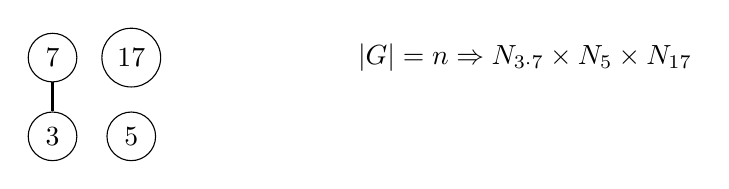
\begin{tikzpicture}
\node[circle,draw] (3) at (0,0) {$3$};
\node[circle,draw] (5) at (1,0) {$5$};
\node[circle,draw] (7) at (0,1) {$7$};
\node[circle,draw] (17) at (1,1) {$17$};

\draw[-,thick] (3) to (7);

\node at (6,1) {$|G|=n\Rightarrow N_{3\cdot 7}\times N_5\times N_{17}$};
\end{tikzpicture}
\end{center}
\end{block}


\end{frame}
    
\begin{frame}{Extending implications}

Factor $n$ into a \emph{direct hypergraph} $\mathcal{H}(n)$.  (i) \emph{Oriented}
Erd\H{o}s-P\'{a}lfy \emph{hyper-}edges, (ii) exceptions for 
finite nonabelian simple groups.

\begin{block}{Proposition}
    A group $G$ of order $n$ factors as 
\[N_0\ltimes (N_1\ltimes \cdots \ltimes N_{\ell}),\] 
$|N_i|=n_i$, where $n_i$ is order of interconnected components of $\mathcal{H}(n)$. 
\end{block}

\pause
\begin{block}{Example $n=5,810,340$}
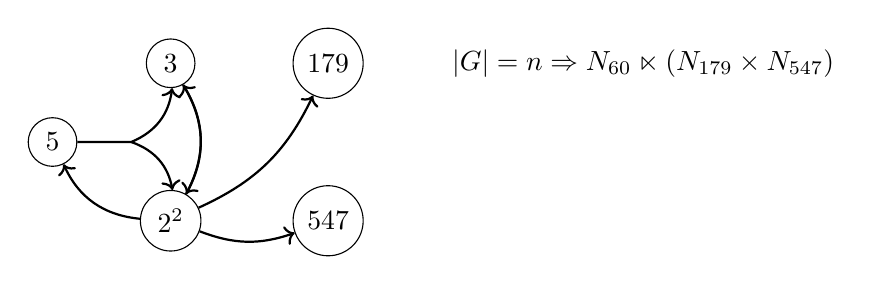
\begin{tikzpicture}
\node[circle,draw] (2) at (0,-1) {$2^2$};
\node[circle,draw] (3) at (0,1) {$3$};
\node[circle,draw] (5) at (-1.5,0) {$5$};
\node[circle,draw] (179) at (2,1) {$179$};
\node[circle,draw] (547) at (2,-1) {$547$};

\draw[->,thick] (2) to[bend right=30]  (3);
\draw[->,thick] (2) to[bend left=30]  (5);
\draw[->,thick] (2) to[bend right=20] (179);
\draw[->,thick] (2) to[bend right=20] (547);

\draw[->,thick] (5) to (-0.5,0) to[bend right=30] (3);
\draw[->,thick] (-0.5,0) to[bend left=30] (2);

\draw[->,thick] (3) to[bend left=30] (2);


\node at (6,1) {$|G|=n\Rightarrow N_{60}\ltimes (N_{179}\times N_{547})$};

\end{tikzpicture}
\end{block}


\end{frame}

\begin{frame}{Most Orders}

\begin{center}
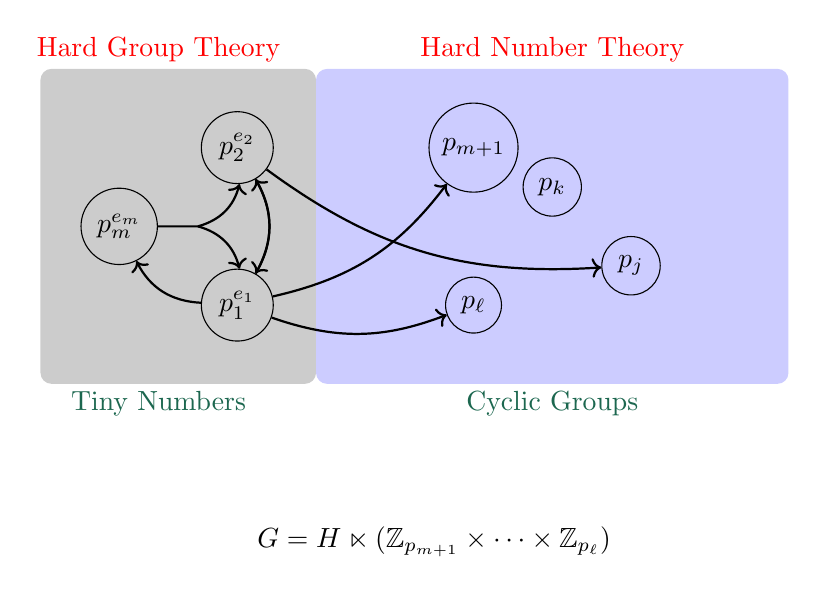
\begin{tikzpicture}

\fill[color=black!20,rounded corners] (-2.5,2) rectangle (1,-2);
\fill[color=blue!20,rounded corners] (1,2) rectangle (7,-2);

\node[circle,draw] (2) at (0,-1) {$p_1^{e_1}$};
\node[circle,draw] (3) at (0,1) {$p_2^{e_2}$};
\node[circle,draw] (5) at (-1.5,0) {$p_m^{e_{m}}$};
\node[circle,draw] (179) at (3,1) {$p_{m+1}$};
\node[circle,draw] (547) at (3,-1) {$p_{\ell}$};
\node[circle,draw] (1949) at (4,0.5) {$p_{k}$};
\node[circle,draw] (7893) at (5,-0.5) {$p_{j}$};



\draw[->,thick] (2) to[bend right=30]  (3);
\draw[->,thick] (2) to[bend left=30]  (5);
\draw[->,thick] (2) to[bend right=20] (179);
\draw[->,thick] (2) to[bend right=20] (547);

\draw[->,thick] (5) to (-0.5,0) to[bend right=30] (3);
\draw[->,thick] (-0.5,0) to[bend left=30] (2);

\draw[->,thick] (3) to[bend left=30] (2);

\draw[->,thick] (3) to[bend right=20] (7893);

\visible<2->{
\node[color=red] at (-1,2.25) {Hard Group Theory};
\node[color=red] at (4,2.25) {Hard Number Theory};
};

\visible<3->{
\node[color=csugreen] at (-1,-2.25) {Tiny Numbers};
\node[color=csugreen] at (4,-2.25) {Cyclic Groups};
\node at (2.5,-4) {$G=H\ltimes (\mathbb{Z}_{p_{m+1}}\times\cdots \times \mathbb{Z}_{p_{\ell}})$};
};


\end{tikzpicture}    
\end{center}

\end{frame}

% \begin{frame}{}
% \begin{itemize}
%     \item Factor $n=ab$ where prime $p|n$, $p\geq\log \log n$ and not exceptional\footnote{primes strongly connected or involved in identifying a nonabelian simple group} then $p|b$;
%     otherwise $p|a$.
    
%     \item Factor $G=H\ltimes_{\theta} B$ with prime divisors $p>\log \log n$ dividing
%     $|B|$ but not $|H|$ (unless exceptional divisor of finite simple groups).
%     Likewise decompose $\tilde{G}=\tilde{H}\ltimes_{\tilde{\theta}} \tilde{B}$.

%     \item Brute-force decide $H\cong \tilde{H}$.
%     \item Canonical isomorphism $B\cong \mathbb{Z}_b\cong \tilde{B}$ by Group Theory.
%     \item Adjust $\theta$ to match $\tilde{\theta}$ if possible.

% \end{itemize}
% \end{frame}

\begin{frame}{Summary}

\begin{block}{IsGroup nearly linear time}
    Promise-to-decision by transferring group to permutation model.
\end{block}

\begin{block}{GroupIso most orders nearly linear time}
    Split group into
    \begin{center} 
        hard group $\ltimes$ hard numbers 
        = tiny numbers $\ltimes$ cyclic groups.
    \end{center}
    Then standard divide-and-conquer.
\end{block}

\rule{\textwidth}{1pt}
{\tiny Thanks to: Newton Institute (Cambridge, UK) 
EPSRC Grant Number EP/R014604/1, Australian Research Council grant
DP190100317, and Simons Foundation Grant 636189.}
\end{frame}

% \begin{frame}{}

% \begin{block}{Theorem.}
% A positive density of positive integers $n$ has $\Gamma(n)$ such 
% that the 
% \end{block}

% \end{frame}

% \begin{frame}{Most integers factor like this}

    
% \begin{tikzpicture}
% \node[circle,draw] (3) at (0,0) {$3$};
% \node[circle,draw] (31) at (1,1) {$31$};
% \node[circle,draw] (137) at (1,-1) {$137$};
% \node[circle,draw] (379) at (2,-1) {$379$};
% \node[circle,draw] (1949) at (3,0) {$1949$};

% \draw[->,thick] (3) to[bend left=30] (0,0.5) to[bend right=30] (31);
% \draw[->,thick] (3) to[bend left=30] (0,0.5) to[bend right=30] (31);
% % \draw[->,thick] (0,0.5) to[bend left=30] (5);
% % \draw[->,thick] (0,0.5) to[bend right=20] (541);

% % \draw[->,thick] (5) to[bend right=30] (-0.25,-0.5) to[bend right=30] (3);
% % \draw[->,thick] (-0.25,-0.5) to[bend left=30] (2);

% % \draw[->,thick] (3) to[bend right=30] (2);


% % \node at (6,1) {$|G|=n\Rightarrow N_{60}\ltimes N_{541}$};

% \end{tikzpicture}
    
% \end{frame}

\end{document}